\begin{figure}[htbp]
  \centering
  \begin{subfigure}{0.8\linewidth}
  \centering
  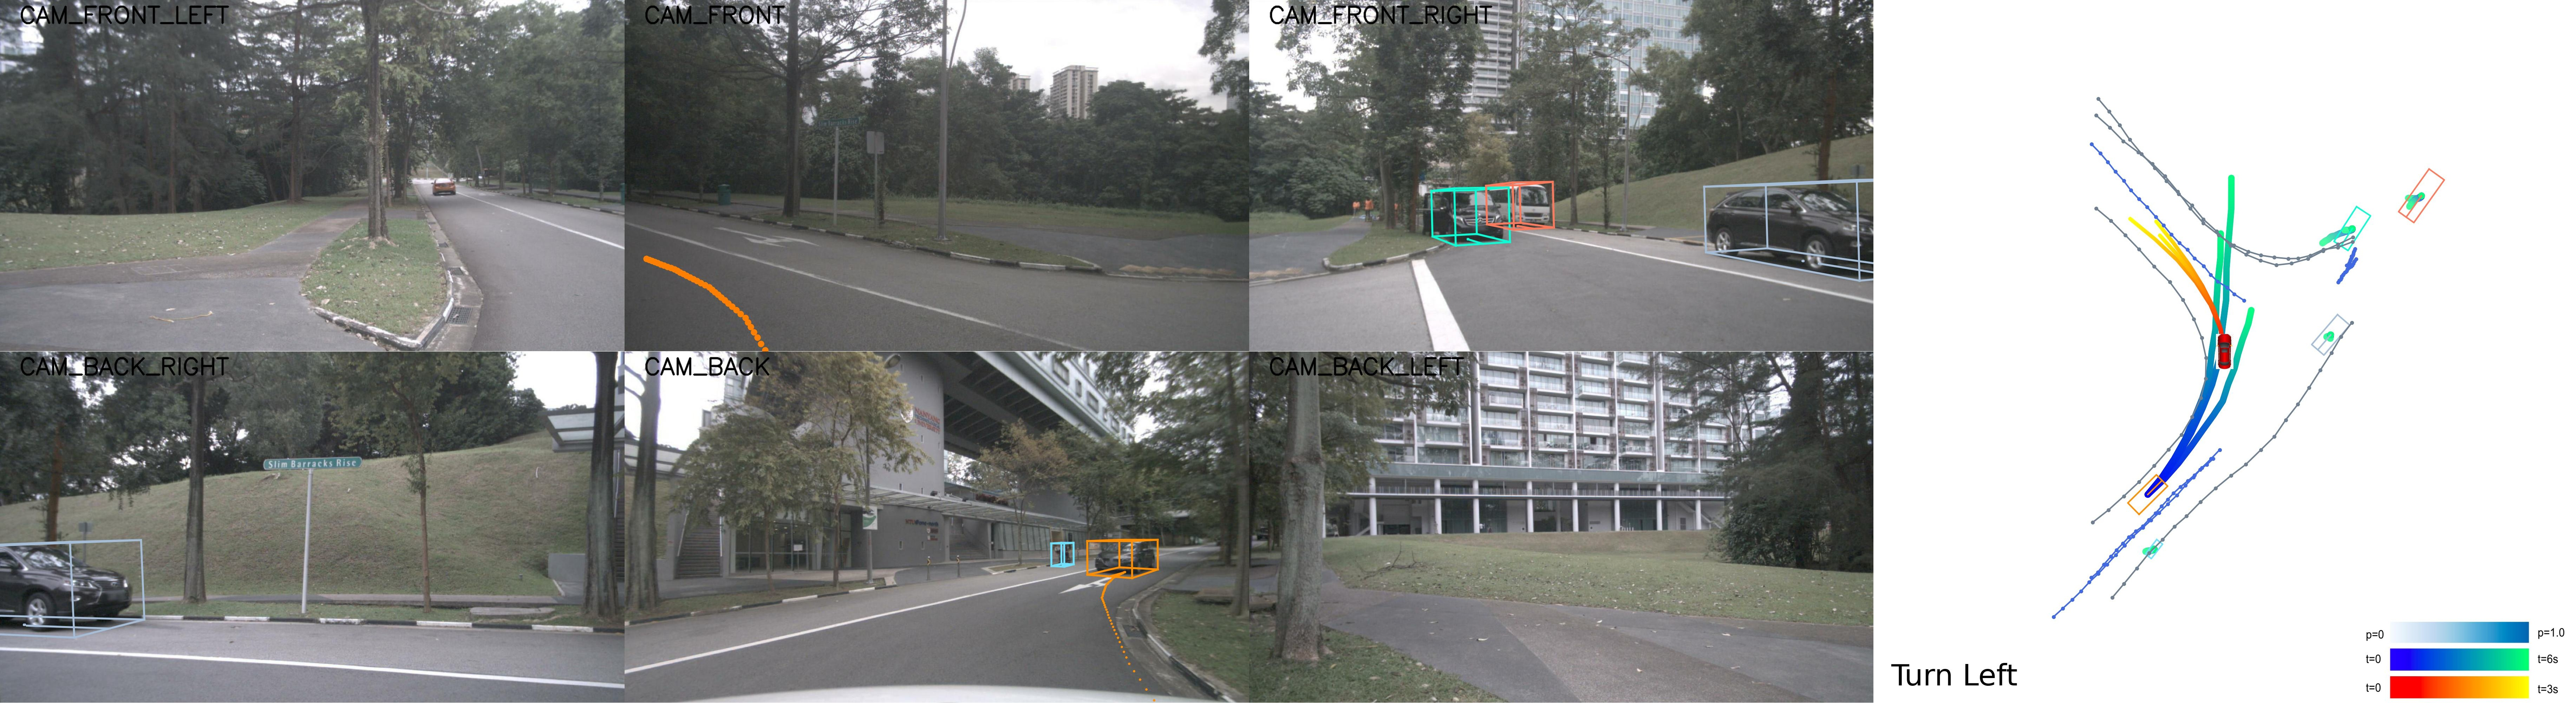
\includegraphics[width=1.0\linewidth]{Figures/vis/turn1.jpg}
  \end{subfigure}
  \begin{subfigure}{0.8\linewidth}
  \centering
  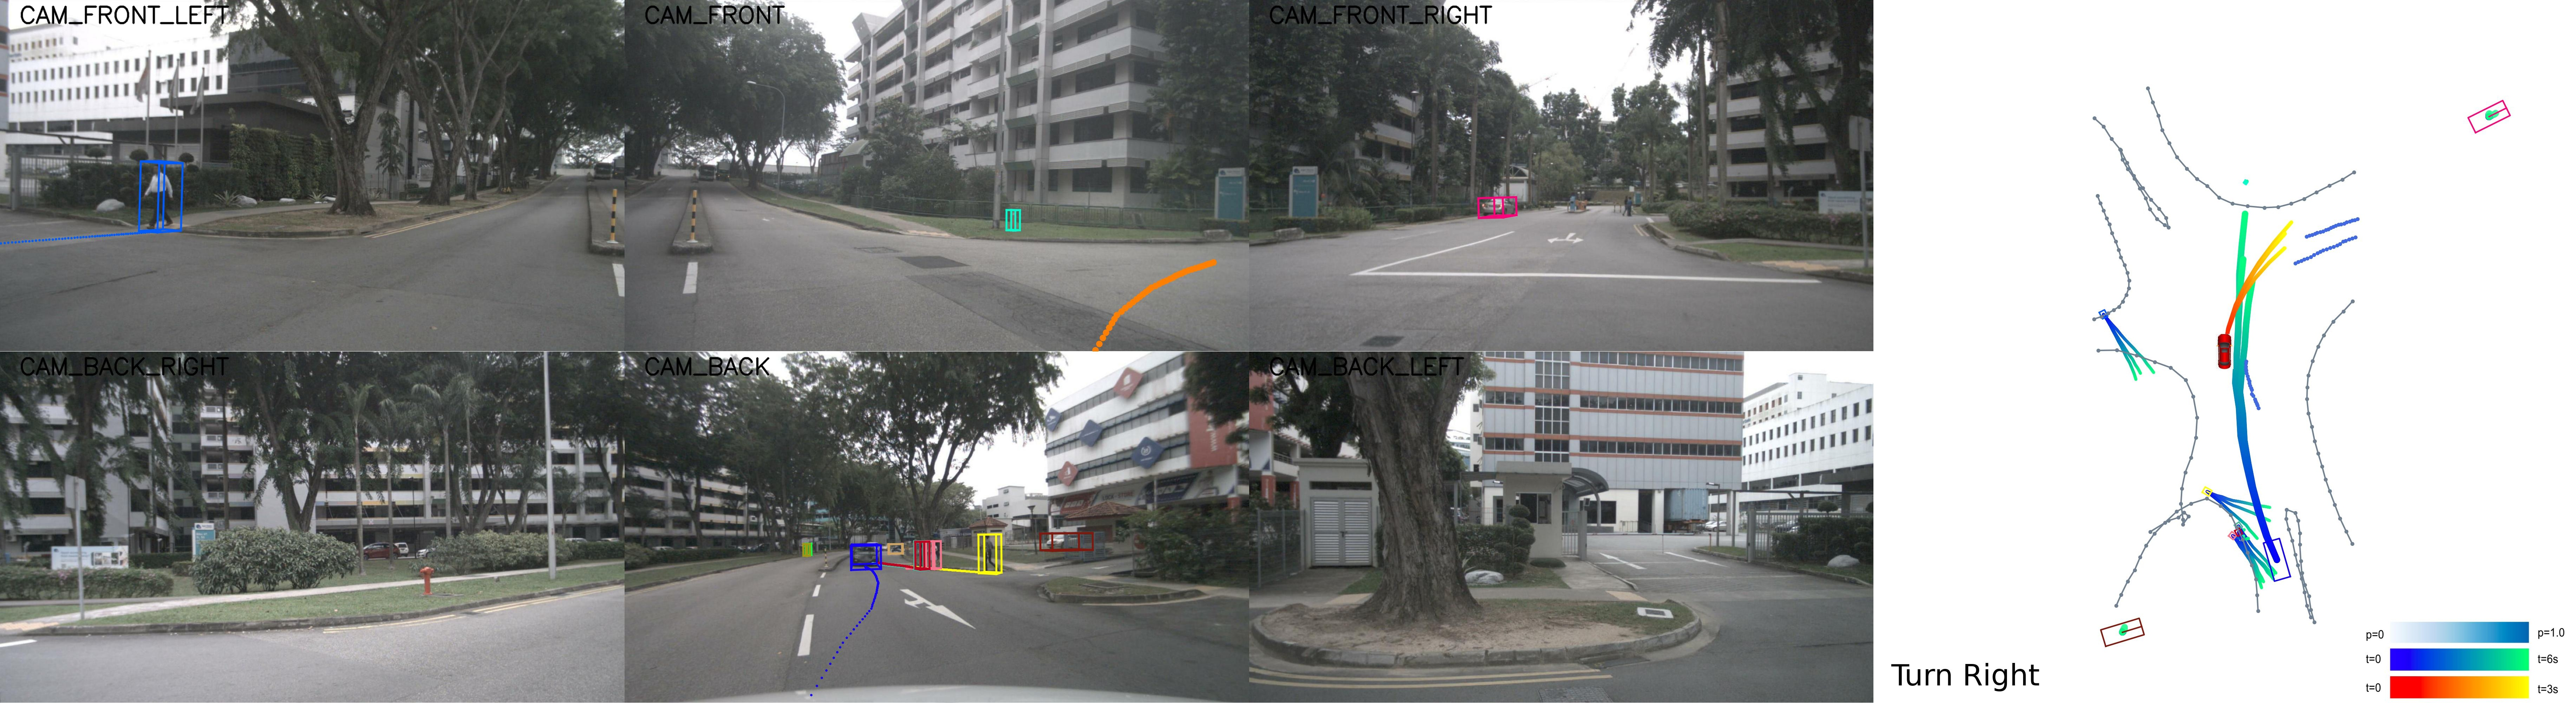
\includegraphics[width=1.0\linewidth]{Figures/vis/turn2.jpg}
  \end{subfigure}
  \begin{subfigure}{0.8\linewidth}
  \centering
  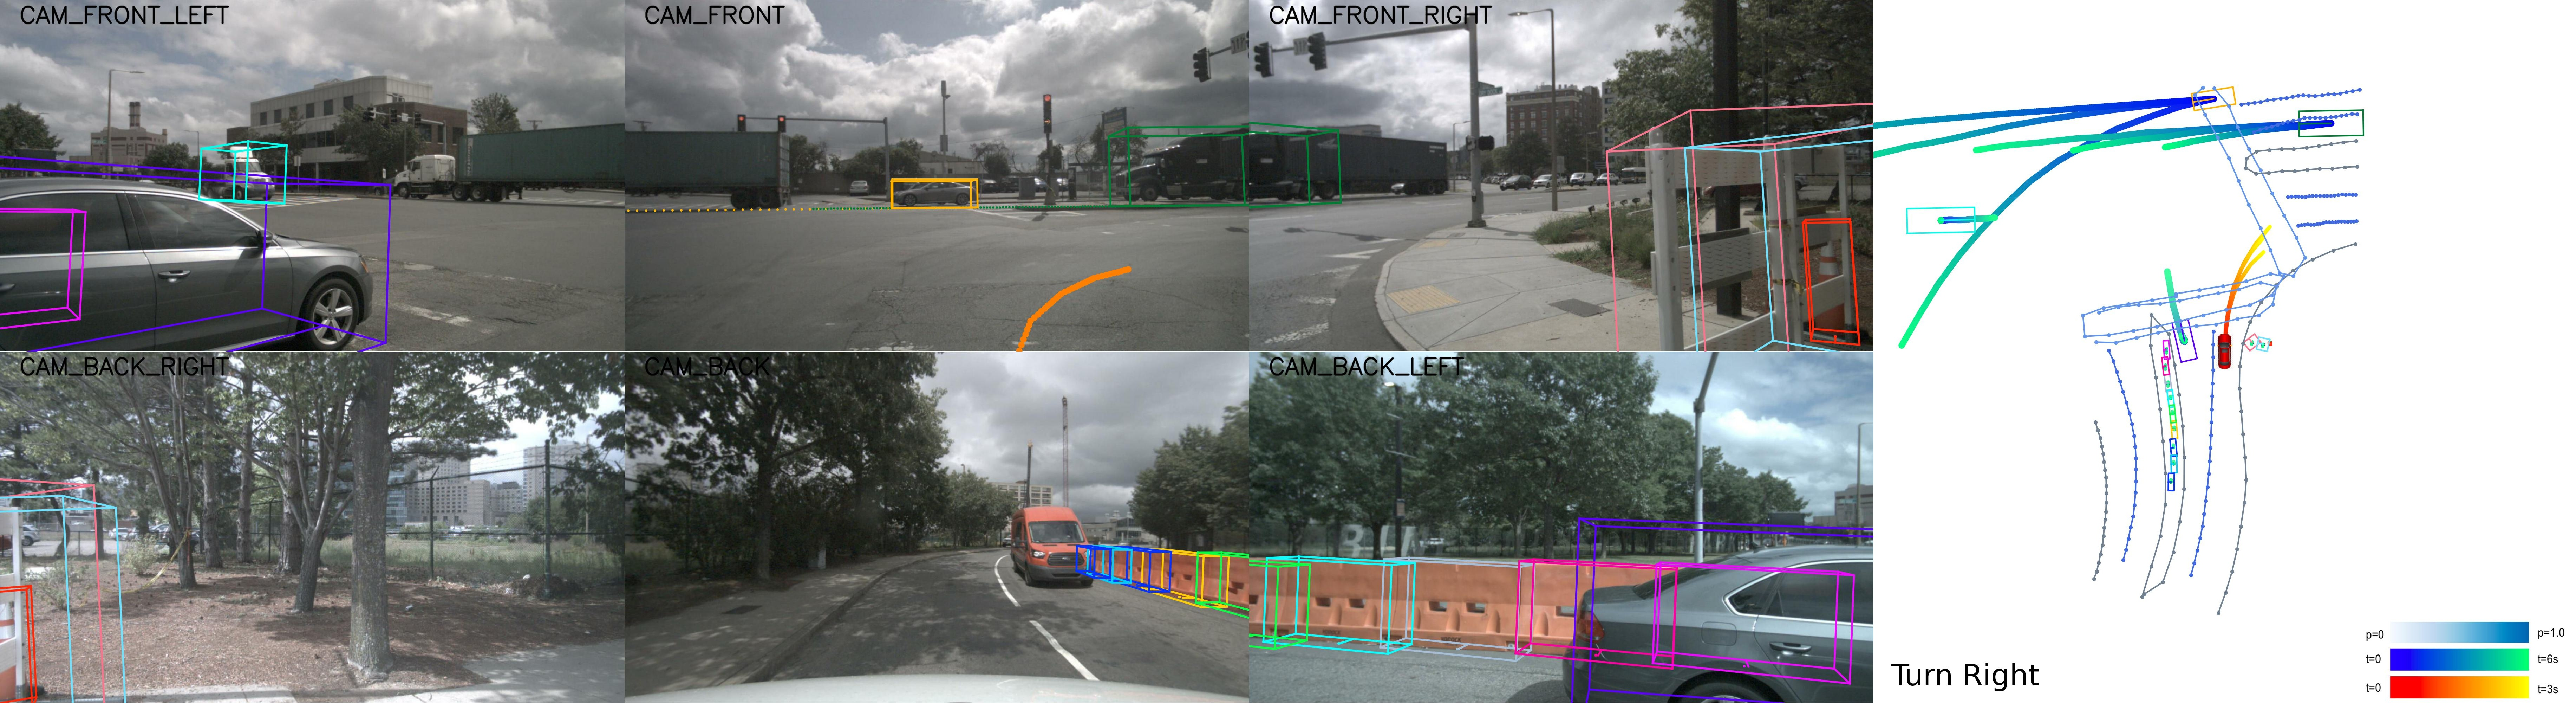
\includegraphics[width=1.0\linewidth]{Figures/vis/turn3.jpg}
  \end{subfigure}
  \begin{subfigure}{0.8\linewidth}
  \centering
  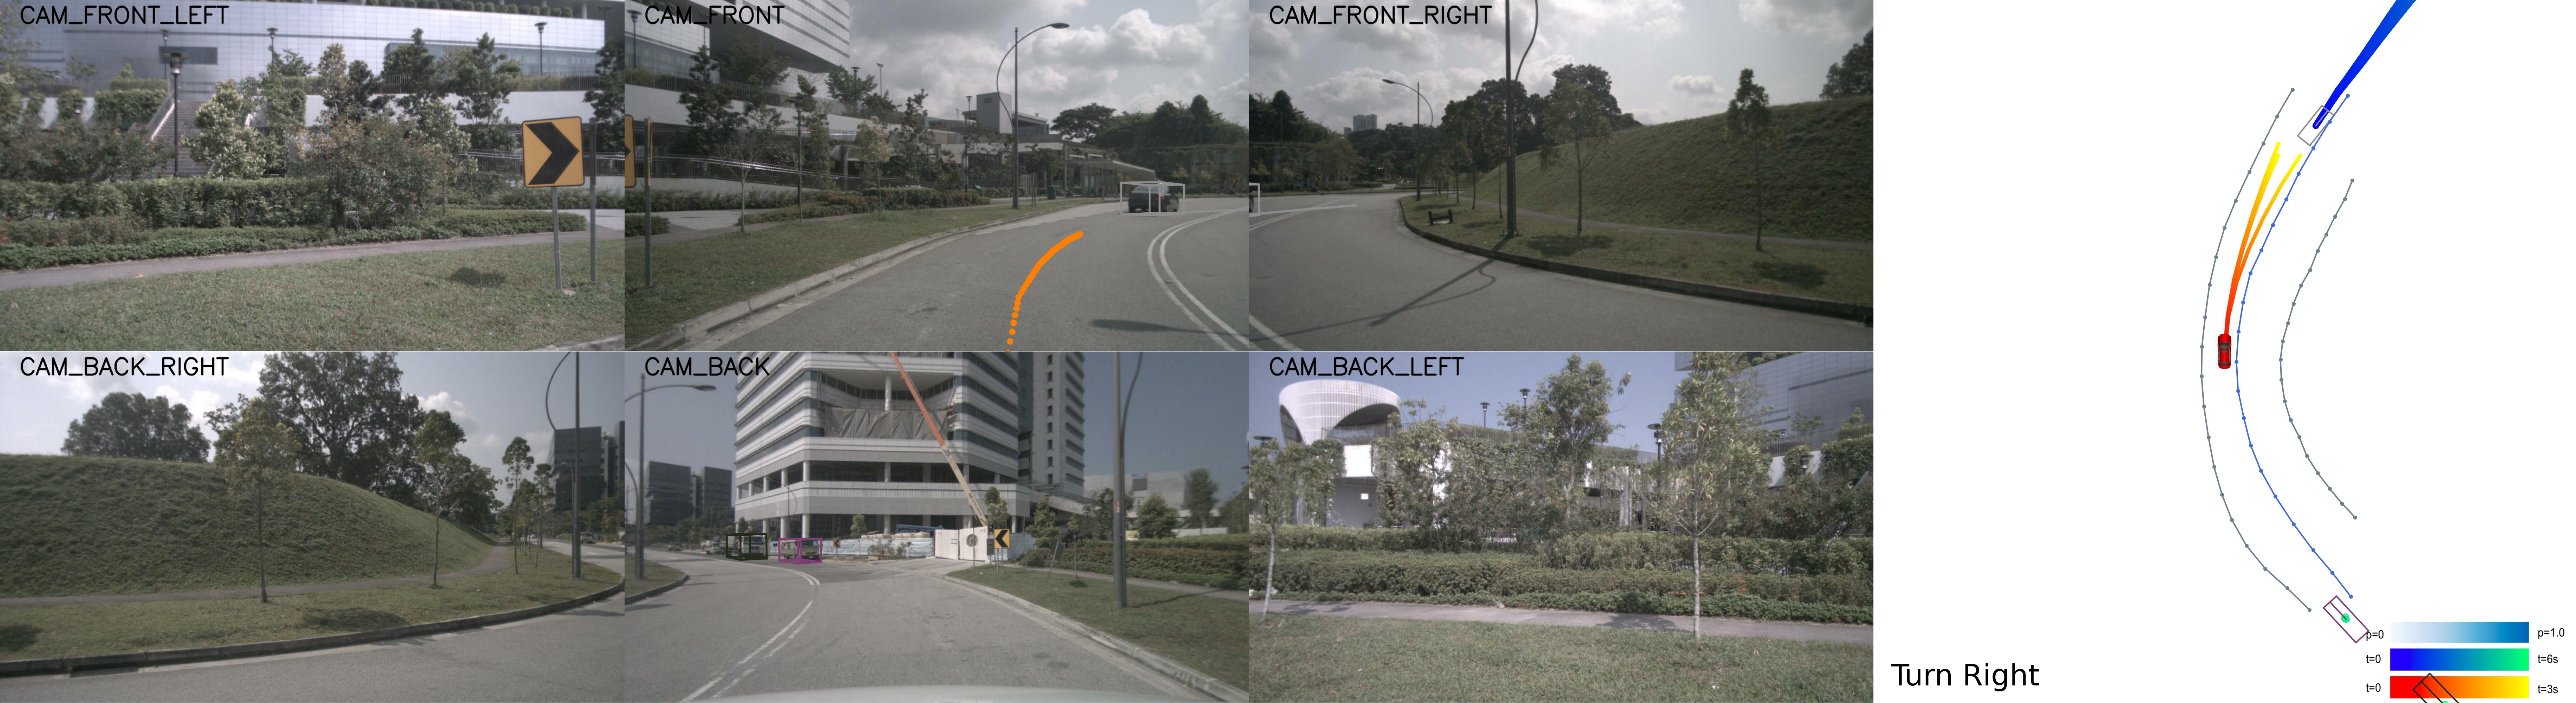
\includegraphics[width=1.0\linewidth]{Figures/vis/turn4.jpg}
  \end{subfigure}
  \caption{Visualization results. SparseDrive learnes different turning modes at intersections.}
  \label{fig:vis}
\end{figure}